\documentclass[12pt]{article}
\usepackage[per-mode=fraction]{siunitx}
\usepackage[margin = 1in]{geometry}
\usepackage{subfigmat}
\usepackage{graphicx}
\usepackage[numbered]{mcode}
\usepackage{multirow}
\usepackage[hidelinks=true]{hyperref}
\usepackage[noabbrev]{cleveref}
\usepackage[section]{placeins}

\author{Nick Stockton}
%\supervisor{Dr. Kelly Cohen}
\title{A Genetic Fuzzy Approach to Controlling the F4 Fighter Jet in Approach Condition}
\date{\today}

\newcommand{\matlab}{\textsc{Matlab}}

\renewcommand{\arraystretch}{2}

\newcommand{\testdir}{test}

\begin{document}
\maketitle
\section{Introduction}
The main challenge of this problem lies in the fact that the flight conditions that a fighter jet experiences are wide and varied. It is simply not possible to design and implement an optimal controller for each on specifically. In this situation, it is logical to design a controller which works near optimally for those conditions which the jet is likely to spend a lot of time in, but one which also works for the flight conditions at the edge of the envelope. The traditional approach for this desired behavior is to determine the PID gains for each common flight condition and perform gains scheduling to allow the controller response to be tuned to each condition. This works quite well for most situations, however, it also presents some downsides. Firstly, gains scheduling necessarily happens with less frequency than the control loop; this means that there will be times during transitions in flight conditions in which the gains used in the control loop are different than the optimal gains for the controller. Additionally, scheduling gains assumes a discontinuous switch between one flight condition to another, which, in real flight, is actually a smooth transition. An augmentation to traditional gains scheduling is to allow the gains to be set by some higher function so that they can smoothly and constantly ``float'' around to match the flight conditions. One such method is to set the PID gains from a fuzzy inference system (FIS). This paper outlines one such system for the approach condition of an F4 fighter jet. A fuzzy-PID controller was tuned for the nominal approach condition, and then applied to various other flight conditions to show its robustness. The controller was tuned using a genetic algorithm.

\section{Why Fuzzy?}
Fuzzy Logic is well suited to problems where uncertainties and approximations are prevalent. This is a result of the two main parts of a FIS working together to map inputs to outputs: the rule base, and the data base. Together, these two pieces are known as a fuzzy knowledge base. The rule base, made up of linguistic IF-THEN statements, easily translates human expert intuition into computational machine language, while the data base, consisting of fuzzy membership sets, allows inputs to be fuzzified for rule evaluation, and then defuzzified once more to be processed in the system as crisp data. This unique setup allows for complex mappings from inputs to output which would otherwise require difficult, nonlinear equations. This highly nonlinear behavior makes fuzzy systems ideal for controlling equally nonlinear systems, such as the F4 fighter jet. The plants provided for this project all have poles which are very close to the right half of the plane, meaning that this system can easily be destabilized by exerting incorrect control force. Much care needs to be taken when designing a controller for such a system. Fuzzy logic is well-suited to this task in that it will allow the control gains to move around in a way which will keep the poles in the left half of the plane.

One large downside to fuzzy systems are that they require a significant expense of effort to tune. This task becomes even more cumbersome with an increase of membership functions, which, in turn, increase the number of rules (possibly exponentially). The FIS designer is then relegated to either drawing on a store of heuristic knowledge or experience (perhaps from an expert), or to trial-and-error iteration to incrementally improve the controller. The method used in this paper is a GA which plays the part of automating and guiding the trial-and-error process (see next section). This method effectively circumvents te difficulty of tuning a FIS, and makes the job of controlling this near-unstable system more feasible.

\section{System Controller Design Methodology}
At first, an attempt was made to utilize Simulink\textsuperscript{\textregistered} and \textsc{Matlab}\textsuperscript{\textregistered} to design a genetic algorithm (GA) which would simulate the plant transfer functions with a fuzzy-PID controller in the feedback loop. The GA, written in \textsc{Matlab}, would call the Simulink model and evaluate the performance of the controller. This methodology presented a number of problems to the designer. The Simulink Fuzzy Logic Block seemed to slow down the execution of the control loop siginificantly, making a single simulation run up to an order of magnitude slower than one with only PID control. This shortcoming can be circumvented by using a lookup table in place of the fuzzy controller, but the overhead time needed to generate the lookup table negates the simulation speed gains.

In light of the issues with using a Simulink GA, the GA was implemented in traditional \textsc{Matlab} using \verb|ODE45| as the ordinary differential equation solver. Unfortunately, within a single time step of an \verb|ODE45| solution, many steps are taken. This means that it is hard, or impossible, to accurately obtain error derivative and integral terms for use in the PID controller. This led the author to eventually write his own simple ode solver in \textsc{Matlab} which gives access to all erros at each time step, but the execution of a single simulation was expectedly and prohibitively slow.

\begin{figure}[h]
	\centering
	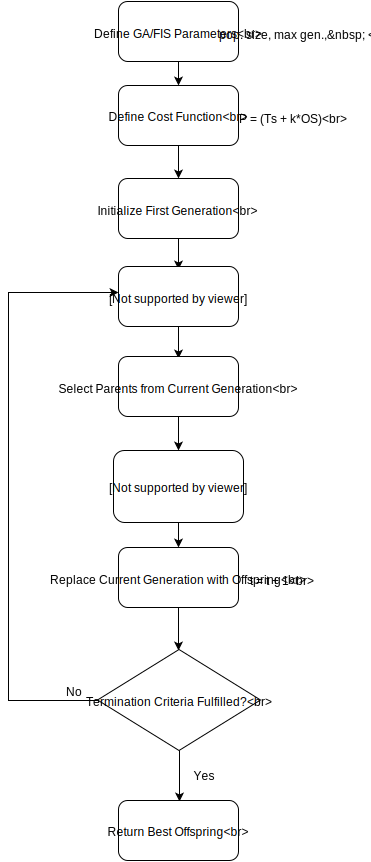
\includegraphics[width=0.5\textwidth]{GA.pdf}
\end{figure}

At this point, the decision was made to implement a genetic fuzzy system using  the C programming language. The author had already implemented one such system in Python and made quick work of translating it into C. This GA uses the comparable rk8pd (Runge-Kutta Prince-Dormand (8,9)) stepping function from the Gnu Scientific Library (GSL) to solve the ordinary differential equation. This method allows the user to specify some basic parameters which are desired in the final FIS, a cost function to be applied to each solution, and some basic parameters for the GA, at which point the GA starts generating and evaluating FIS's until a suitable stop condition has been met.

For this problem, it was determined that a 3-input, 3-output FIS would be suitable to define the PID gains. As input, the FIS accepts the absolute error in elevator position ($e_p$), the error integral ($e_i$), and the error derivative ($e_d$). As output, the FIS generates the Proportional, Derivative and Integral gains ($K_p$, $K_i$, $K_d$). Ideally, one separate FIS for each gain would be deployed with each accepting either error and error derivative, or the corresponding error for each gain (i.e. $e_i\rightarrow K_i$, etc.) The added complexity of tuning three FIS's in parallel was perceived to be too large of an additional cost to algorithm development in exchange for the decoupling of gains definition, so a single FIS was designed in its stead. 

The cost function used to evaluate each FIS was derived using the fuzzy-PID controlled dynamic system response to a step function. The cost function is obtained by simply summing the settling time and the overshoot fraction. It should be noted that likely due to some small numerical differences in the GSL sovler and \textsc{Matlab}'s \verb|ODE45|, the settling times reported by \textsc{Matlab} are merginally slower in most cases than than what is given in \cref{t:f4}.

\section{Results for Nominal and Other Flight Conditions}
\begin{figure}[h]
	\centering
	\begin{subfigmatrix}{2}
	\subfigure[\label{f:f4_nominal}Nominal approach condition]{\includegraphics[width=0.49\textwidth]{results/f4_approach}}
	\subfigure[\label{f:f4_degraded}Degraded aerodynamic derivative approach condition]{\includegraphics[width=0.49\textwidth]{results/f4_deg}}
	\subfigure[\label{f:f4_subsonic}Subsonic cruise condition]{\includegraphics[width=0.49\textwidth]{results/f4_sub}}
	\subfigure[\label{f:f4_supersonic}Supersonic cruise condition]{\includegraphics[width=0.49\textwidth]{results/f4_sup}}
	\end{subfigmatrix}
	\caption{Step response for various flight conditions. Note the increased overshoot for nominal conditions from the Fuzzy-PID controller.}\label{f:f4}
\end{figure}

\begin{table}[h]
	\centering
	\caption{Comparison table of current results with those of Bossert and Cohen}\label{t:f4}
	\begin{tabular}{|c|c|c|c|c|c|}\hline
	Case & $T_s$ (s) & $T_r$ (s) & $T_p$ (s) & $M_p$ (deg) & FV (deg) \\\hline
	Root Locus F4 Approach (Design Condition) & 23.6 & 1.09 & 3.14 & 1.09 & 0.62 \\\hline
	PID F4 Approach (Design Condition) & 7.08 & 1.27 & 4.98 & 1.023 & 1.00 \\\hline
	Fuzzy F4 Approach (Design Condition) & 1.65 & 1.68 & 1.74 & 1.013 & 1.00 \\\hline
	\textbf{Fuzzy PID Approach (Design Condition)} & 1.86 & 0.26 & 0.66 & 1.396 & 1.00\\\hline

	Root Locus 50\% Red in $C_{m\alpha}$ and $C_{mq}$ & 25.8 & 1.16 & 3.57 & 1.42 & 0.77 \\\hline
	PID 50\% Red in $C_{m\alpha}$ and $C_{mq}$ & 8.0 & 1.03 & 1.35 & 1.045 & 1.01 \\\hline
	Fuzzy 50\% Red in $C_{m\alpha}$ and $C_{mq}$ & 1.66 & 1.69 & 1.75 & 1.014 & 1.00 \\\hline
	\textbf{Fuzzy PID 50\% Red in $C_{m\alpha}$ and $C_{mq}$} & 4.47 & 0.33 & 0.66 & 1.043 & 1.00\\\hline

	\end{tabular}
\end{table}

\begin{figure}[h]
	\centering
	\begin{subfigmatrix}{2}
	\subfigure[\label{f:f4_nominal_nos}Nominal approach condition]{\includegraphics[width=0.49\textwidth]{results/\testdir/f4_approach}}
	\subfigure[\label{f:f4_degraded_nos}Degraded aerodynamic derivative approach condition]{\includegraphics[width=0.49\textwidth]{results/\testdir/f4_deg}}
	\subfigure[\label{f:f4_subsonic_nos}Subsonic cruise condition]{\includegraphics[width=0.49\textwidth]{results/\testdir/f4_sub}}
	\subfigure[\label{f:f4_supersonic_nos}Supersonic cruise condition]{\includegraphics[width=0.49\textwidth]{results/\testdir/f4_sup}}
	\end{subfigmatrix}
	\caption{Step response for various flight conditions. Note the significantly decreased overshoot for nominal and degraded flight conditions.}\label{f:f4_nos}
\end{figure}

\begin{table}[h]
	\centering
	\caption{Resulting FIS response from GA with modified cost function}\label{t:f4_nos}
	\begin{tabular}{|c|c|c|c|c|c|}\hline
	Case & $T_s$ (s) & $T_r$ (s) & $T_p$ (s) & $M_p$ (deg) & FV (deg) \\\hline
	Fuzzy PID Approach (Design Condition) & 1.86 & 0.26 & 0.66 & 1.396 & 1.00\\\hline

	Fuzzy PID 50\% Red in $C_{m\alpha}$ and $C_{mq}$ & 4.47 & 0.33 & 0.66 & 1.043 & 1.00\\\hline

	\end{tabular}
\end{table}

\begin{table}[h]
	\centering
	\caption{Comparison of response times for subsonic and supersonic cruise conditions for original and modified cost function. Modifying the cost function showed no improvements for this set of conditions, rather only proved to slow the response time with no gain in overshoot.}\label{t:subsup}
	\begin{tabular}{|c|c|c|c|c|c|}\hline
	Case & $T_s$ (s) & $T_r$ (s) & $T_p$ (s) & $M_p$ (deg) & FV (deg) \\\hline
	Subsonic Cruise (Orig. Cost) & 0.93 & 0.38 & 3.91 & 1.022 & 1.00\\\hline

	Supersonic Cruise (Orig. Cost) & 3.84 & 0.73 & 11.10 & 1.018 & 1.01\\\hline

	Subsonic Cruise (Mod. Cost) & 0.93 & 0.38 & 3.91 & 1.022 & 1.00\\\hline

	Supersonic Cruise (Mod. Cost) & 15.53 & 0.73 & 11.74 & 1.020 & 1.00\\\hline

	\end{tabular}
\end{table}

\section{Discussion}
As can be seen from \cref{t:f4} and \crefrange{f:f4_nominal}{f:f4_degraded}, the overshoot which comes at a cost of decreased settling time is unacceptable. This is a product of defining a cost function which under-penalizes overshoot and over-emphasizes settling time alone. The results were retained as part of the project to show both the benefits and shortcomings of using a GA t tune a FIS. That is, the FIS will be shaped to minimize the cost of whatever function is provided, whether or not the desired outcome is truly reflected by that function. For this reason, much care is needed when choosing a cost function to be minimized. The GA was given a new cost function which put a higher premium on overshoot and given a FIS to optimize for the plant. The results from this run are shown in \cref{t:f4_nos} and \cref{f:f4_nos}. As can be seen from \cref{t:f4_nos}, the settling time of the step response is significantly slower, but the overall response is arguably better that \cref{f:f4} due to the reduced overshoot. Additionally, though not nearly as good for the nominal and degraded flight conditions as was Bossert and Cohen's solution, the response for the subsonic and supersonic cruise conditions show arguably better performance than theirs.

\section{Conclusion}
It has been shown that fuzzy augmented systems can greatly improve the behavior of controllers. Where traditional control logic can attain reasonable performance for only nominal and near-nominal conditions, fuzzy logic can extend the performance gains across a much wider set of conditions.

For future work, the genetic fuzzy library is going to be modified to be able to incorporate the tuning and learning of multiple FIS's in parallel. This would allow for the decoupling of the output gains for this system, which may improve the settling time of the response while maintaining an acceptable overshoot. This new library will also allow for the generation of cascaded fuzzy systems which are useful in many applications where the solution space might otherwise grow to unmanageable sizes. Also, some work will be done to further improve the speed of execution of the C library. Much care was taken to execute only the fewest essential steps in evaluating a FIS as possible, but there are some improvements to be made yet.

\end{document}